\section{Results} \label{sec:results}

\Cref{table:results-selected-model} shows the average performance of the
selected model in the \nameref{subsubsec:evaluatio-dataset} dataset.
\Cref{fig:high-slip} shows its results on an evaluation recording characterized
by high slippage driving conditions.

\begin{table}
    \centering
    \begin{tabular}{|c|c|c|}
        \hline
                        & Mean ATE [m] & Mean RPE [m] \\ \hline
        All microphones & $1.02e-03$   & $5.10e-03$     \\
        \hline
    \end{tabular}
    \caption[Selected model average performance across evaluation recordings
        and microphones]{Selected model average performance across all
        evaluation recordings and averaged across all microphones. Absolute
        Trajectory Error (ATE) is computed between frames with a duration of
        15 ms and Relative Pose Error (RPE) \cite{Measuring2019} is computed
        using time windows 1 s long.}
    \label{table:results-selected-model}
\end{table}


\begin{figure*}
    \centering
    \begin{tikzpicture} \node [anchor=south west] at (0,0) {
            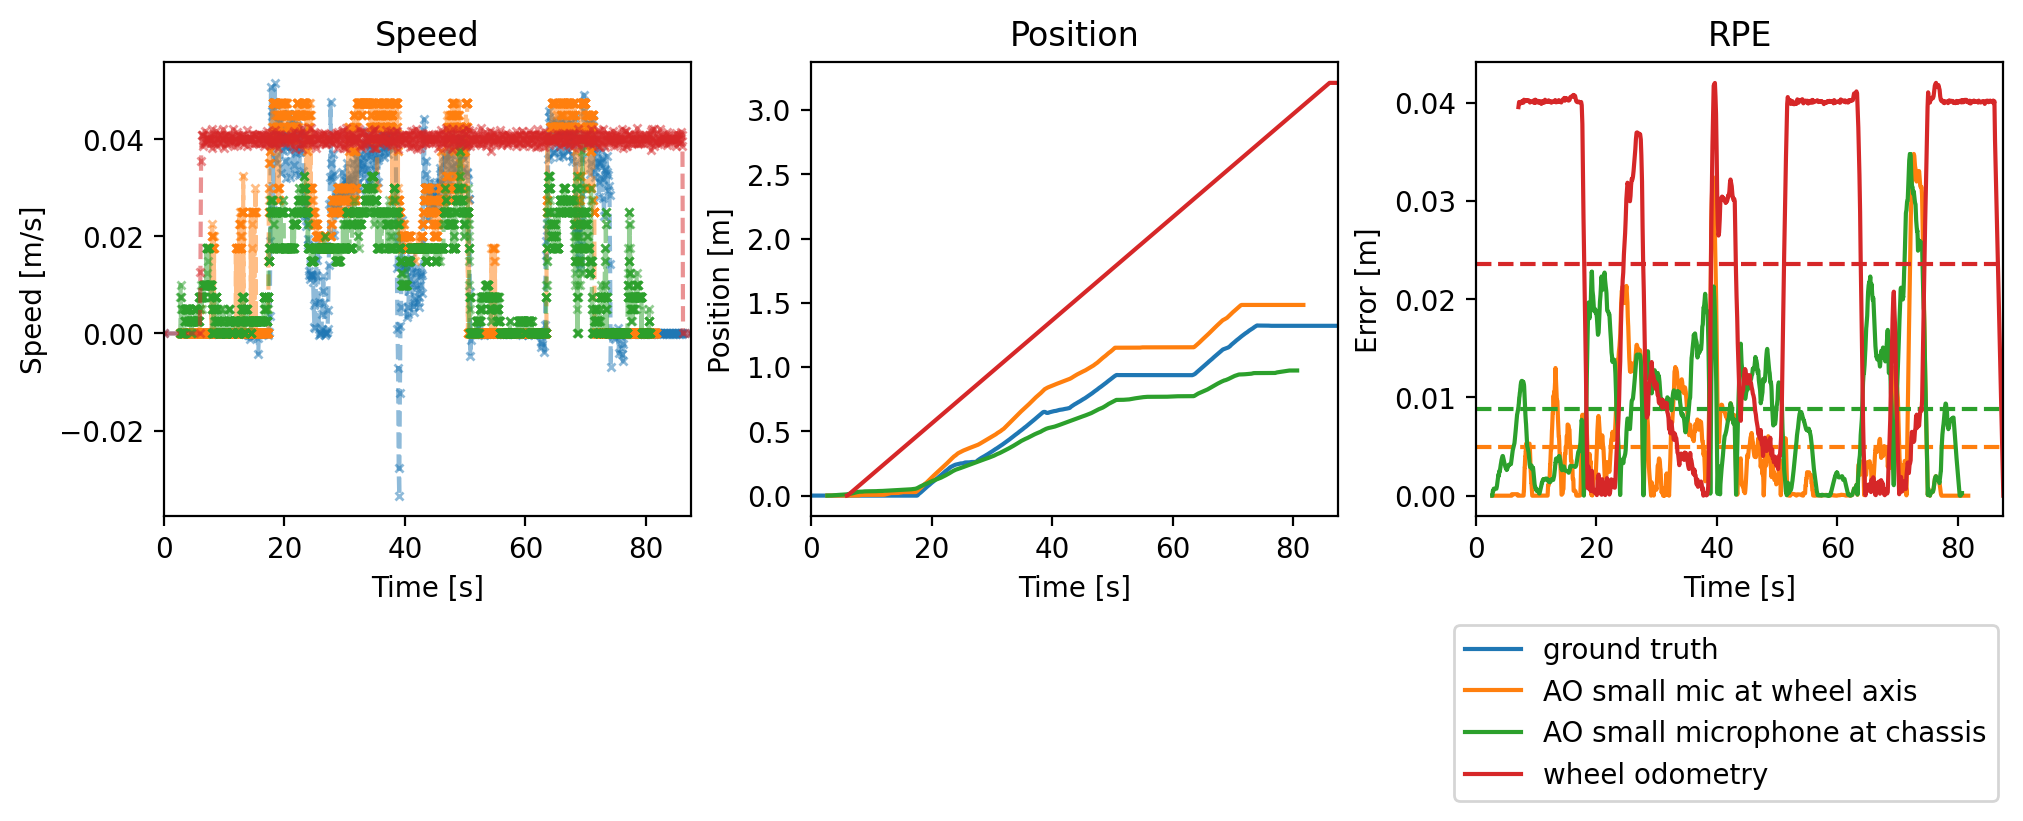
\includegraphics[width=.95\textwidth]{\subdir/high-slip.png}
        }; \node [anchor=south west, text width=.65\textwidth] at (0,-1) {
            \caption{Evaluation of a recording characterized by high slippage
            conditions. The left figure shows longitudinal velocity estimated
            using the selected model (\emph{AO}), the measured wheel angular
            velocity (\emph{wheel odometry}) and position (\emph{ground
            truth}). The integrated longitudinal position is shown in the
            center figure. The right figure shows the evolution of the Relative
            Pose Error \cite{Measuring2019} computed using time windows 1 s
            long.}
            \label{fig:high-slip}
        }; \end{tikzpicture}
\end{figure*}

% Review33: The authors state "Generally, white noise increases the value of
% the estimated motion." why is that?

\subsection{Noise} The selected model has been evaluated in the same recording
shown in \cref{fig:high-slip} in the presence of synthetic white noise of
varying signal-to-noise ratio values. Noise with the same power as the signal
(SNR 0 dB) increases the mean Relative Pose Error 2.62\%. SNR of -10 dB affects
significantly the predictions at low speeds and when the robot is not moving
increasing the RPM a 38.91\%.

% \begin{figure*}
%     \centering
%     \begin{tikzpicture} \node [anchor=south west] at (0,0) {
%             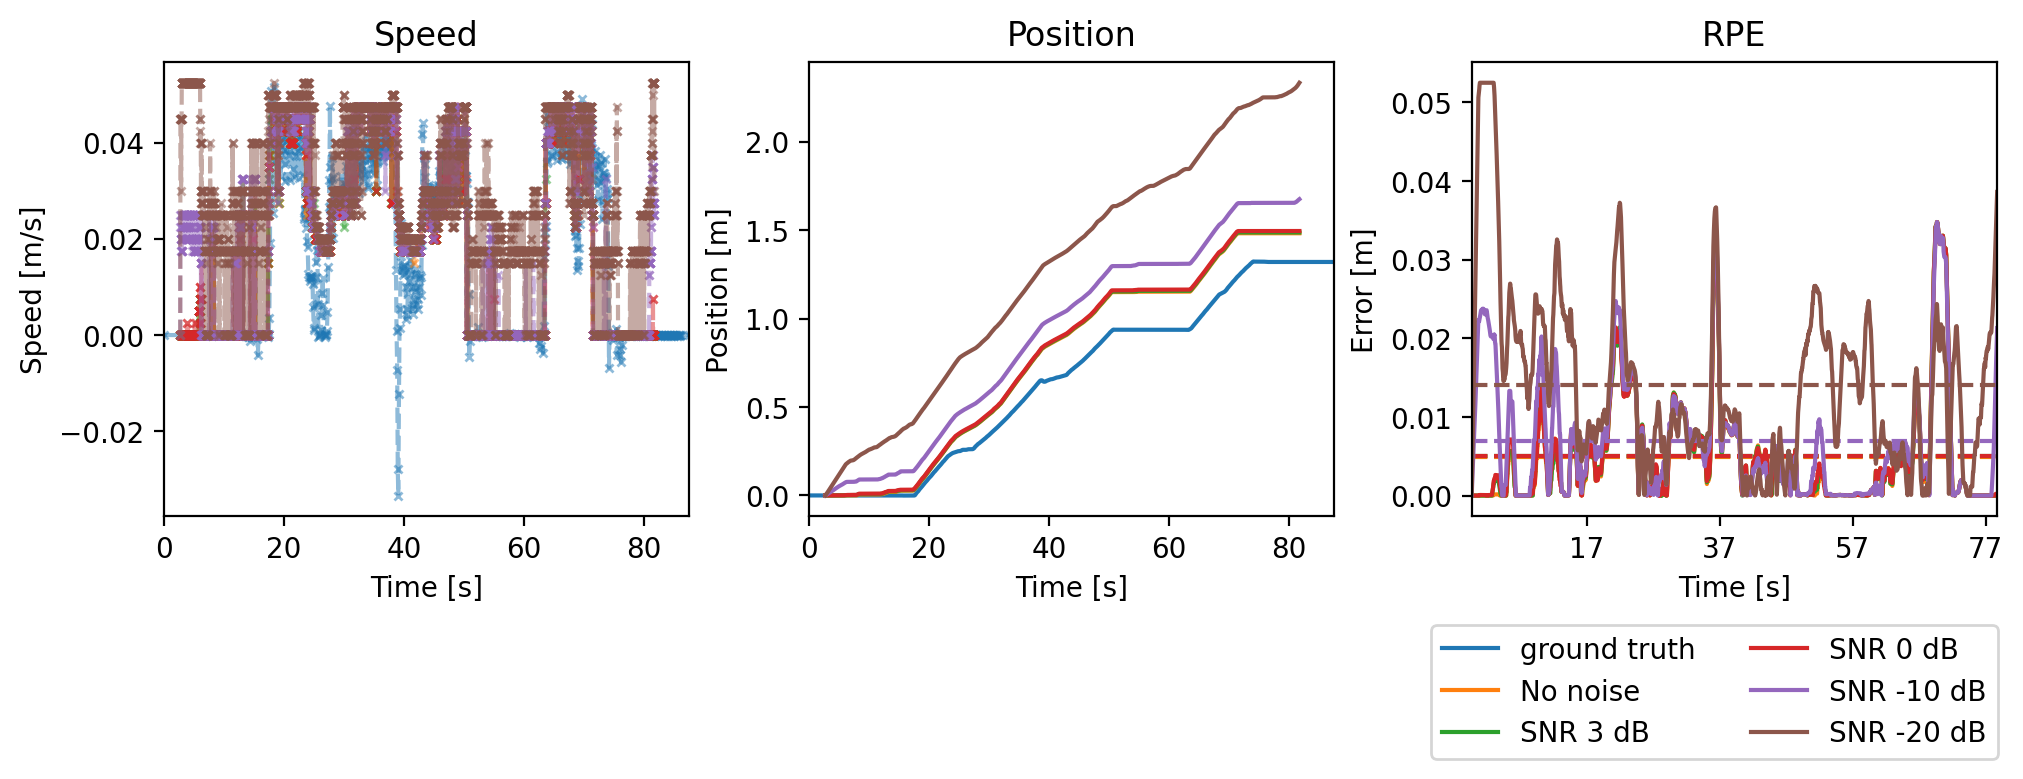
\includegraphics[width=.95\textwidth]{\subdir/noise-effect.png}
%         }; \node [anchor=south west, text width=.65\textwidth] at (0,0.2) {
%             \caption{Selected model evaluated on the same recording as
%             \cref{fig:high-slip} with added white noise with varying
%             signal-to-noise ratio values.}
%             \label{fig:noise-effect}
%         }; \end{tikzpicture}
% \end{figure*}

\subsection{Computational cost} Tests with the selected model on a CPU show
that the time to compute the feature extraction is a 40\% of the total time to
process a new frame, which is 2.03 ms on an Intel\textregistered{}
Core\texttrademark{} i7-9750H CPU at 2.60GHz. The prediction time takes up a
55\% of the total time while the remaining 5\% corresponds to loading the new
frame into memory. The system is able to run 7.5 times faster than real time on
this particular hardware. Using hardware acceleration with CUDA the total time
to process a new frame is slightly lower: 1.93 ms on a NVIDIA GeForce RTX 2060
GPU.

\subsection{Compared with other models} The selected model is evaluated against
two other odometry methods: Wheel odometry computed from the measured wheel
angular velocity; and Intel\textregistered{} RealSense\texttrademark{} Tracking
Camera T265, which is based on visual odometry. \Cref{fig:other-methods} is the
evaluation in an ideal scenario for all methods. \Cref{fig:VO-challenge}
instead corresponds to a scenario that is challenging for visual odometry.
Dynamic objects are moved in the camera field of view and lightning conditions
are changed during the recording. One can see in this evaluation that the
vulnerabilities of audio-based odometry and visual-based odometry do not
overlap.

\begin{figure*}
    \centering
    \begin{tikzpicture} \node [anchor=south west] at (0,0) {
            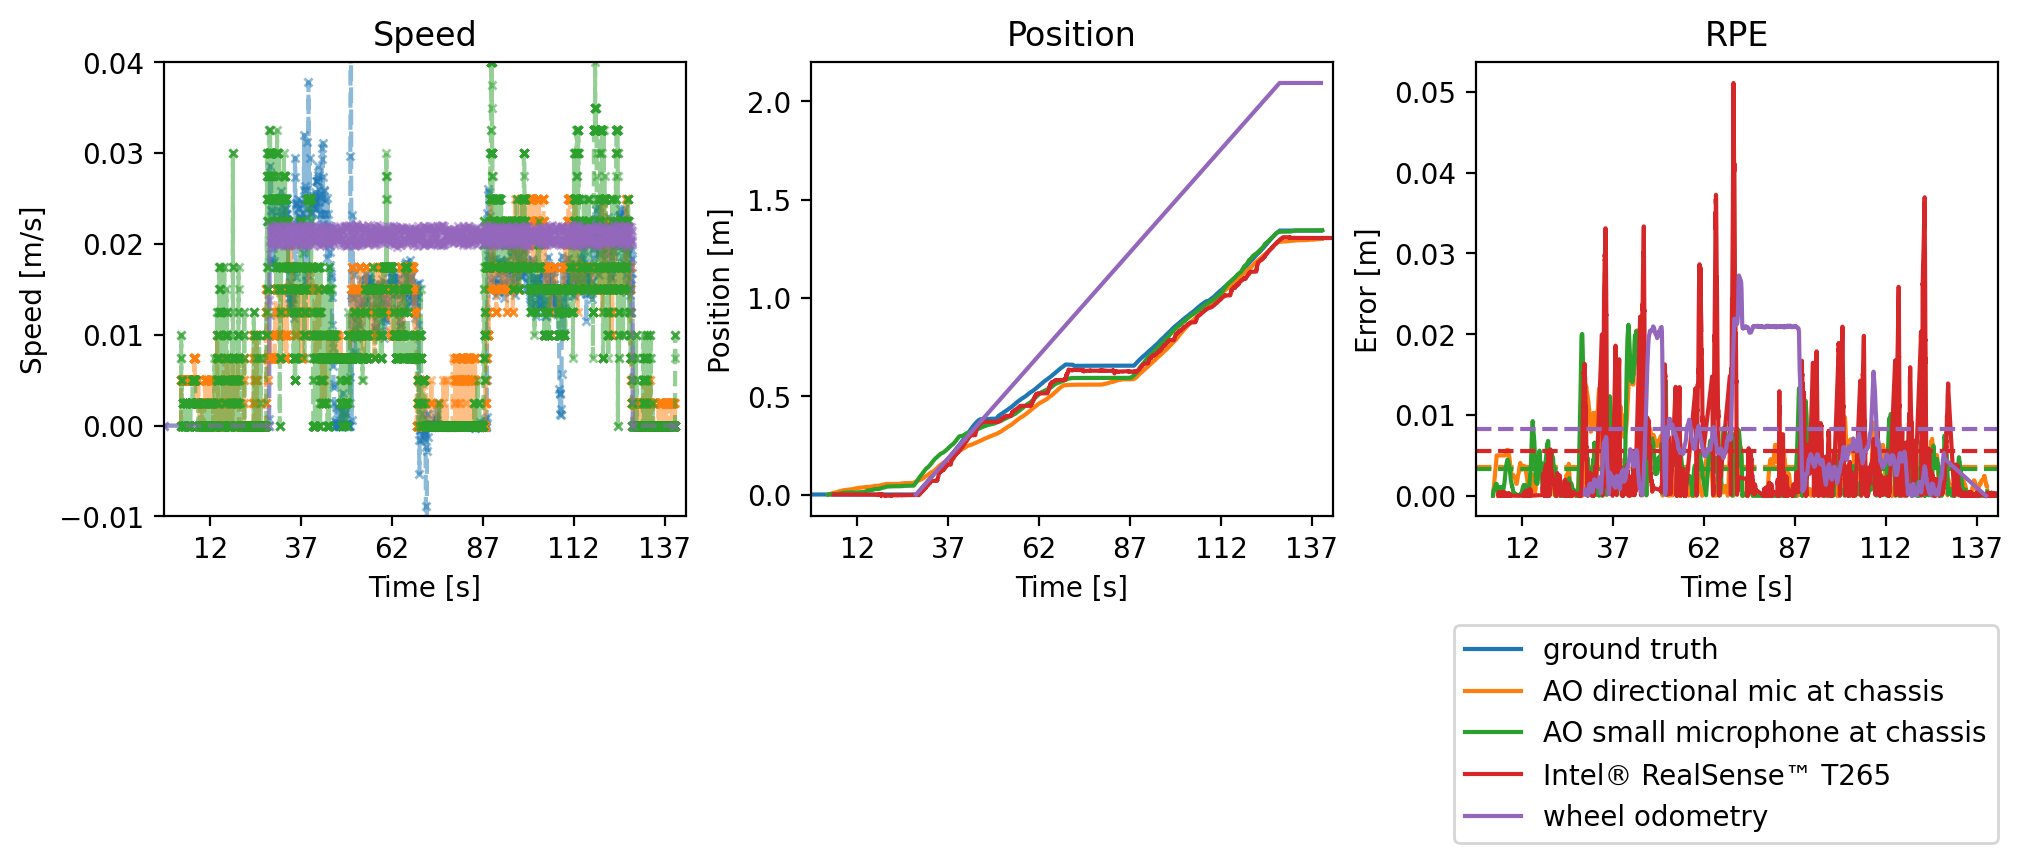
\includegraphics[width=.95\textwidth]{\subdir/other-methods.png}
        }; \node [anchor=south west, text width=.65\textwidth] at (0,0) {
            \caption{Selected model evaluated evaluated against wheel odometry
            and Intel\textregistered{} RealSense\texttrademark{} Tracking
            Camera T265 (based on visual odometry). One can see in the central
            figure that the proposed system can perform with an accuracy
            comparable to commercially available visual-based systems in this
            simplified scenario.}
            \label{fig:other-methods}
        }; \end{tikzpicture}
\end{figure*}

\begin{figure*}
    \centering
    \begin{tikzpicture} \node [anchor=south west] at (0,0) {
            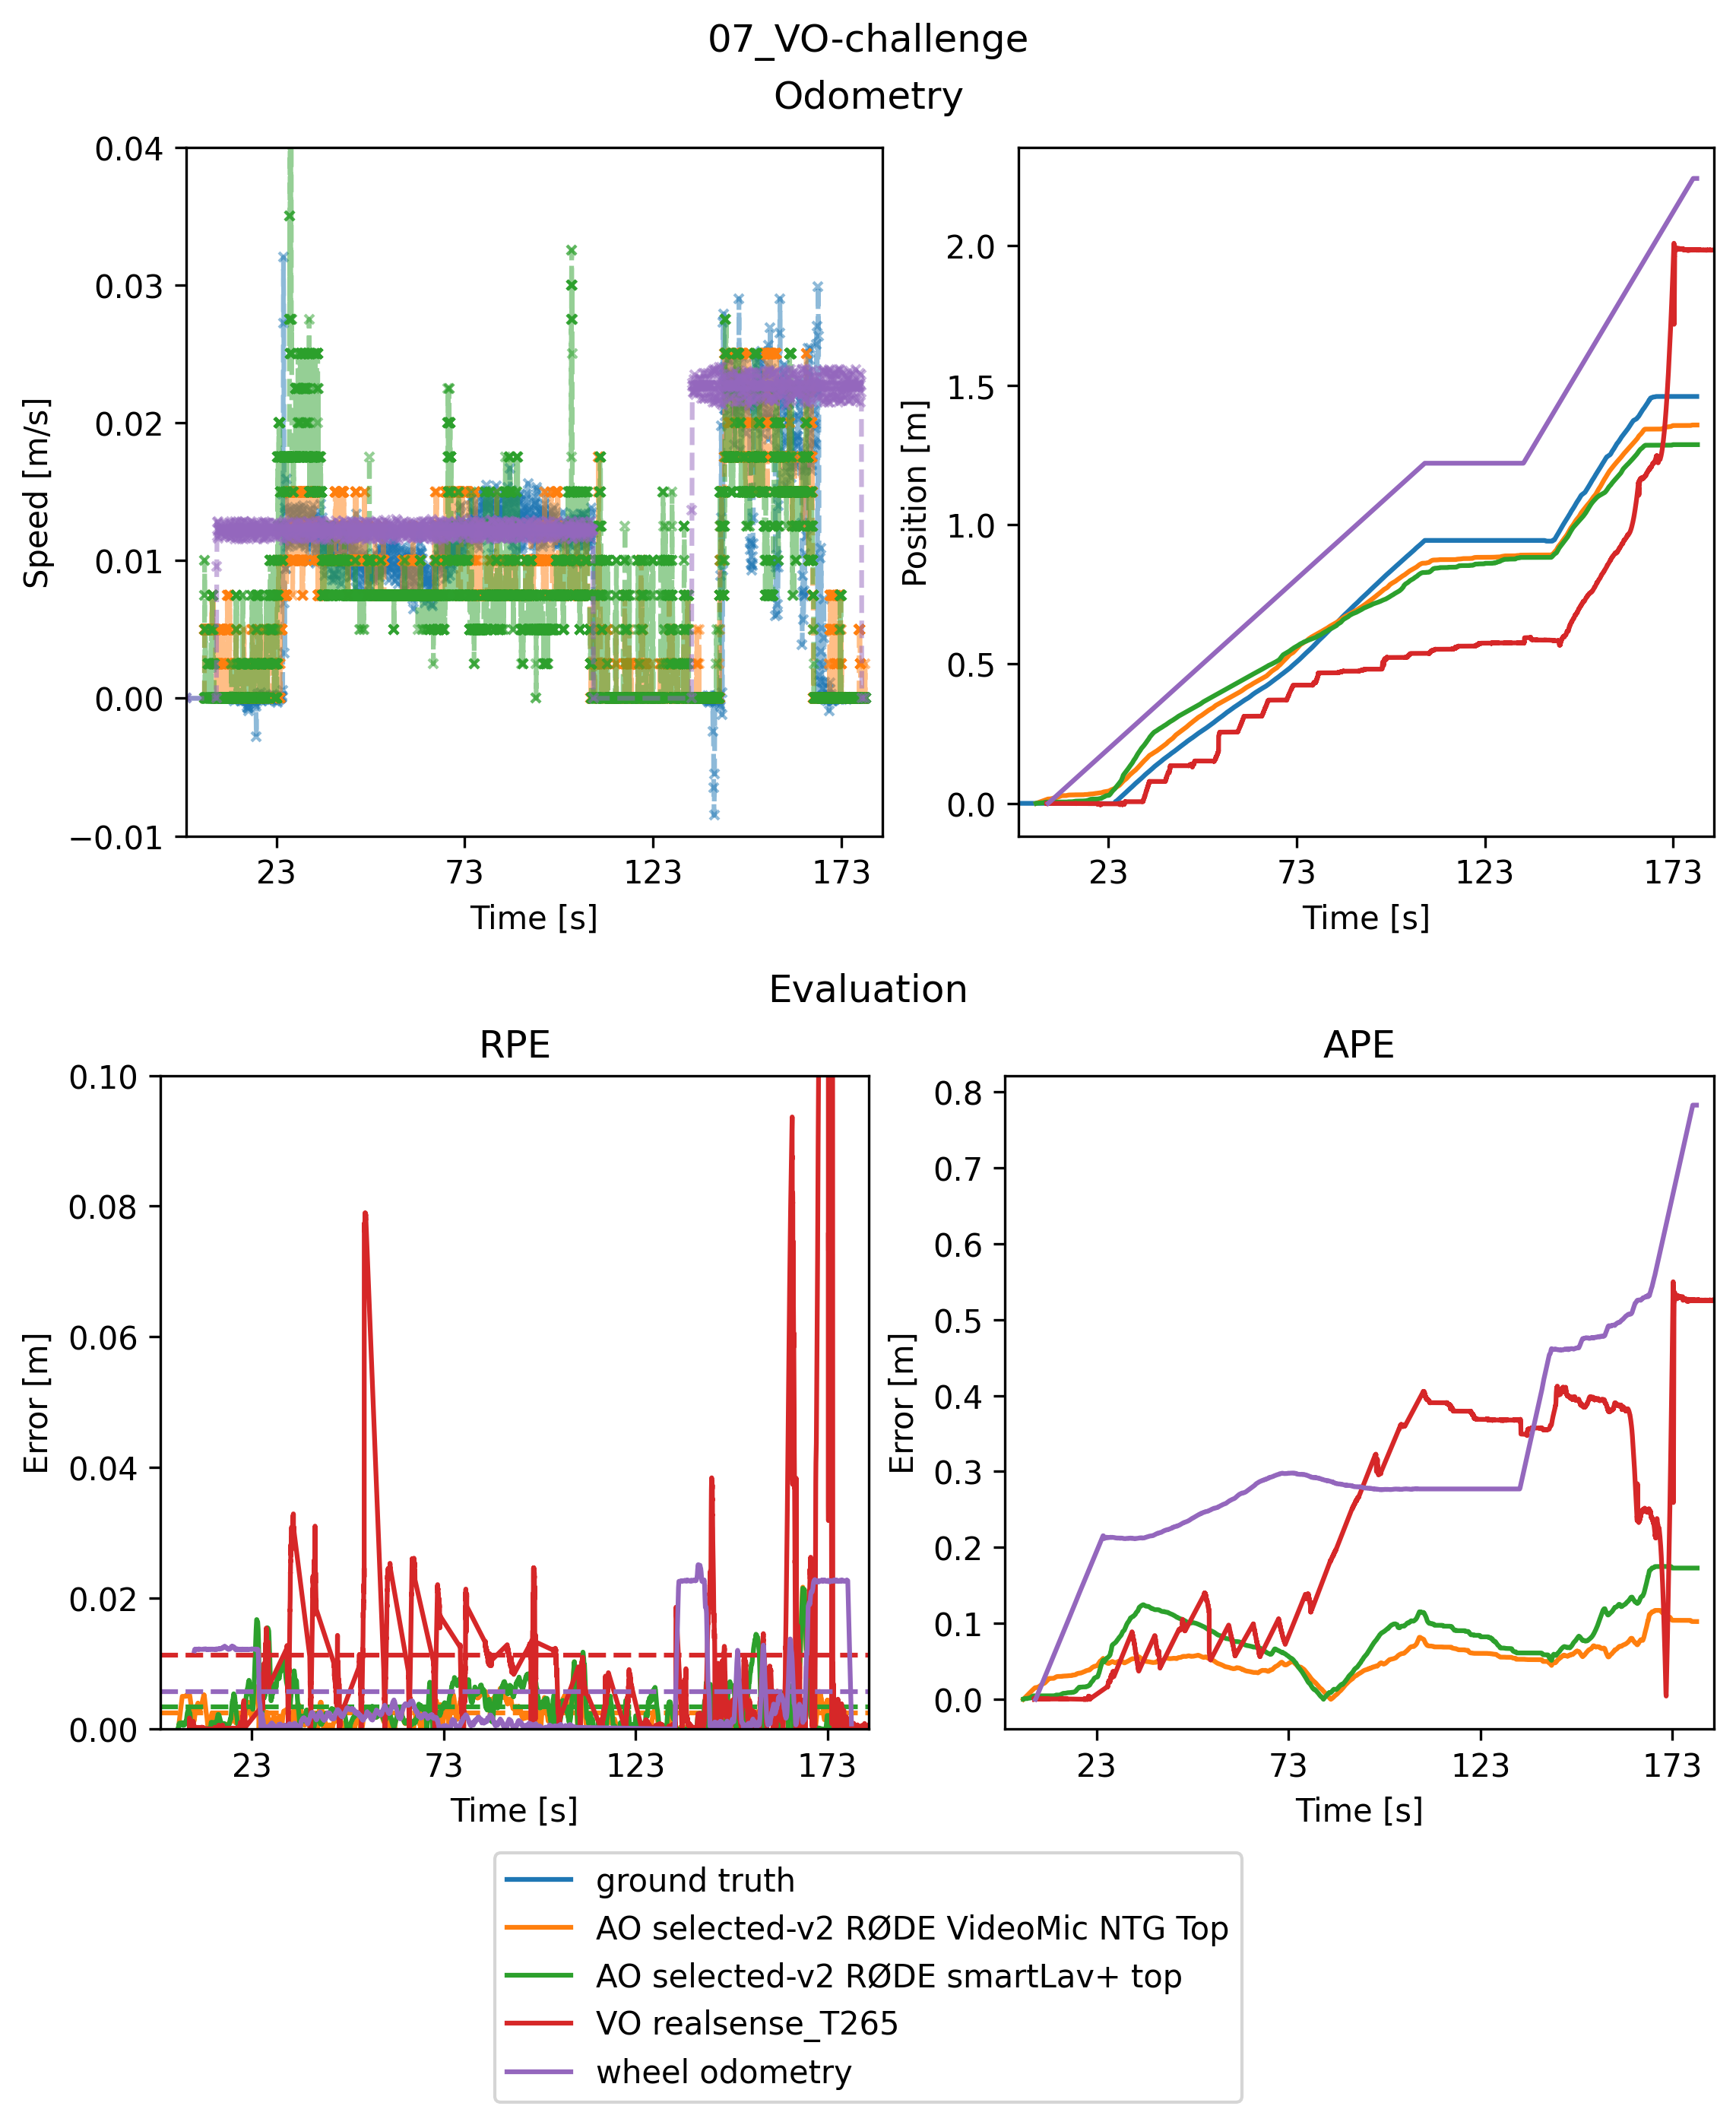
\includegraphics[width=.95\textwidth]{\subdir/VO-challenge.png}
        }; \node [anchor=south west, text width=.65\textwidth] at (0,0) {
            \caption{Selected model evaluated against Intel\textregistered{}
            RealSense\texttrademark{} Tracking Camera T265 (based on visual
            odometry) in a scenario where visual odometry vulnerabilities are
            exploited: Dynamic objects are moved in the camera field of view
            and lightning conditions are changed during the recording.}
            \label{fig:VO-challenge}
        }; \end{tikzpicture}
\end{figure*}

\include*{\subdir/discussion}